% This is part of Un soupçon de mathématique sans être agressif pour autant
% Copyright (c) 2012
%   Laurent Claessens, Pauline Klein
% See the file fdl-1.3.txt for copying conditions.

%+++++++++++++++++++++++++++++++++++++++++++++++++++++++++++++++++++++++++++++++++++++++++++++++++++++++++++++++++++++++++++
\section{Introduction, domaine de définition}
%+++++++++++++++++++++++++++++++++++++++++++++++++++++++++++++++++++++++++++++++++++++++++++++++++++++++++++++++++++++++++++


\begin{example} \label{ExemVmCkIH}
    Un petit tour de magie. Choisissez un nombre entre \( 1\) et \( 10\). Ajoutez \( 5\), multipliez par \( 2\), ajoutez \( 7\), enlevez le double du nombre de départ.

    Le nombre que vous avez maintenant est \( 17\).
\end{example}

\begin{definition}
    Soit \( \defD\) un ensemble de nombres. On définit une \defe{fonction}{fonction} \( f\) sur \( \defD\) en associant à chaque nombre \( x\) dans \( \defD\) un seul nombre \( y\). Dans ce cas nous disons que \( f\) est une fonction de la \defe{variable}{variable} \( x\).
\end{definition}

La partie difficile de cette définition est l'introduction du domaine de définition \( \defD\). Oublions la un instant pour comprendre le reste. Sans parler de \( \defD\), la définition s'écrit :

\begin{quote}
    On définit une \defe{fonction}{fonction} \( f\) en associant à chaque nombre \( x\) un seul nombre \( y\).
\end{quote}
Cela n'est rien d'autre qu'une façon savante de dire qu'une fonction «prend un nombre en entrée, fait des calculs et retourne un nombre en sortie».

Pourquoi introduit-t-on le domaine de définition ? Simplement parce que toute fonction ne va pas accepter toutes les valeurs en entrée. Le domaine de définition est l'ensemble des valeurs acceptées.

\begin{example}
    Soit la fonction qui à la longueur d'un segment fait correspondre la surface du carré construit sur ce segment. Cette fonction n'est définie que sur les nombres positifs (parce qu'il n'existe pas de segments de longueurs négatives). Nous écrivons donc
    \begin{equation}
        \begin{aligned}
            f\colon \mathopen[ 0 , \infty [&\to \eR \\
            x&\mapsto x^2,
        \end{aligned}
    \end{equation}
    et nous avons \( f(x)=x^2\).
\end{example}

\begin{example}
    Soit la fonction qui a un nombre entier fait correspondre la somme de ses chiffres. Par exemple \( f(0)=0\) et \( f(123)=6\). Cette fonction est définie sur les entiers et retourne un entier. Nous pouvons écrire
    \begin{equation}
        \begin{aligned}
            f\colon \eN&\to \eN \\
            x&\mapsto f(x). 
        \end{aligned}
    \end{equation}
    Ici il est compliqué de donner une forme explicite pour \( f\).
\end{example}

\begin{example}
    Considérons la fonction qui a un nombre fait correspondre son inverse : \( f(x)=\frac{1}{ x }\). Pour se dérouiller le cerveau, je propose quelque valeurs :
    \begin{equation}
        \begin{aligned}[]
            f(1)&=1&f(5)&=\frac{1}{ 5 }&f(\frac{ 2 }{ 3 })=\frac{ 3 }{ 2 }\\
            f(\frac{ 1 }{ 4 })&=4&f(-3)&=-\frac{1}{ 3 }&f(-1)&=-1.
        \end{aligned}
    \end{equation}
    Cette fonction est implémentée en python de la façon suivante :

\lstinputlisting{ex_inverse.py}

donne

\lstinputlisting[title=Résultat]{res_ex_inverse.txt}

Très clairement, python ne veut pas calculer l'inverse de zéro et plante sur un message on ne peut plus clair : \info{ZeroDivisionError: division by zero}.

Effectivement, l'inverse de zéro n'existe pas. Le domaine de notre fonction \( f(x)=1/x\) n'est donc pas \( \eR\) tout entier, mais seulement \( \eR\setminus\{ 0 \}\).

\end{example}


En ce qui concerne les notations, nous écrivons
\begin{equation}
    \begin{aligned}
        f\colon \defD&\to \eR \\
        x&\mapsto f(x). 
    \end{aligned}
\end{equation}
Cela signifie que \( \defD\) est l'\defe{ensemble de définition de \( f\)}{ensemble!de définition}, c'est à dire l'ensemble des nombres sur lesquels \( f\) peut être appliquée. Le symbole \( \eR\) désigne l'ensemble de tous les nombres.

%+++++++++++++++++++++++++++++++++++++++++++++++++++++++++++++++++++++++++++++++++++++++++++++++++++++++++++++++++++++++++++
\section{Antécédent}
%+++++++++++++++++++++++++++++++++++++++++++++++++++++++++++++++++++++++++++++++++++++++++++++++++++++++++++++++++++++++++++

\begin{Aretenir}
Une fonction associe à chaque nombre de l'ensemble de définition \emph{un seul} nombre, appelé \defe{image}{image}. Si \( a\) est un nombre, un \defe{antécédent}{antécédent} de \( a\) par la fonction \( f\) est un nombre \( x\defD\) tel que 
\begin{equation}
    f(x)=a.
\end{equation}
\end{Aretenir}
Trouver des antécédents revient souvent à résoudre des équations.

Il peut arriver qu'un nombre ait plusieurs antécédents.

\begin{example}
    Pour la fonction \( f(x)=2x-1\), un antécédent de \( 5\) est le nombre \( 3\). Un antécédent du nombre \( -10\) est la nombre \( -9/2\).

    Plus généralement les antécédents de \( a\) sont les solutions de l'équation
    \begin{equation}
        2x-1=a,
    \end{equation}
    c'est à dire \( x=\frac{ a+1 }{2}\).
\end{example}

\begin{example} \label{EqlaIGDz}
    Si nous avons une série statistique de \( n\) valeurs, pour trouver le premier quartile nous devons diviser \( n\) par \( 4\) et prendre l'entier le plus proche vers le haut. Cela donne le numéro de la valeur correspondante au premier quartile.

    En python, la fonction qui donne le numéro de la valeur du premier quartile en fonction de \( n\) est
    \begin{quote}
        \info{math.ceil(n/4)}
    \end{quote}
    Notons \( f\) cette fonction. Son domaine est l'ensemble des entiers non nuls. Le graphique de cette fonction est donné à la figure \ref{LabelFigMathCeilwCXIJZ}.
\newcommand{\CaptionFigMathCeilwCXIJZ}{Le numéro de la valeur du premier quartile en fonction du nombre de valeurs.}
\input{Fig_MathCeilwCXIJZ.pstricks}

    Le graphique est uniquement constitué de points. Pas de lignes entre, parce qu'il n'existe pas de séries statistiques comprenant \( 3.7\) valeurs par exemple. 
\end{example}

\Exo{Seconde-0053}

\begin{example}
    Soit la fonction définie sur \( \defD=\{ -5,-1,1,3,9 \}\) de la façon suivante :
    \begin{equation}
        \begin{array}[h]{|c||c|c|c|c|c|c|}
            \hline
            x&-5&-1&1&3&9&10\\
            \hline
            f(x)&0&2&-3&7&2&5\\
            \hline
        \end{array}
    \end{equation}
    Nous pouvons dire que
    \begin{enumerate}
        \item
            L'image de \( 1\) par \( f\) est \( -3\).
        \item
            L'unique antécédent de \( 7\) est \( 3\).
        \item
            Les nombres \( -1\) et \( 9\) sont tous deux des antécédents de \( 2\).
    \end{enumerate}
\end{example}

\begin{example}
    Soit la fonction \( f(x)=(x+1)^2\). Nous avons \( f(-1)=0\), \( f(4)=25\); nous disons que \( 0\) est l'image de \( -1\) par \( f\) et que \( 25\) est l'image de \( 4\) par \( f\).

    Remarquons que \( f(-2)=1\) et \( f(0)=1\). Donc \( -2\) et \( 0\) sont deux antécédents de \( 1\).
\end{example}

%+++++++++++++++++++++++++++++++++++++++++++++++++++++++++++++++++++++++++++++++++++++++++++++++++++++++++++++++++++++++++++
\section{Modélisation par une fonction}
%+++++++++++++++++++++++++++++++++++++++++++++++++++++++++++++++++++++++++++++++++++++++++++++++++++++++++++++++++++++++++++

Les exemples de fonctions dans la «vraie» vie sont nombreux.

\begin{example}
    Soit un triangle rectangle isocèle dont les côtés de l'angle droit sont de longueur \( x\). Alors la surface est donnée par la fonction
    \begin{equation}
        f(x)=\frac{ x^2 }{2}.
    \end{equation}
    Le domaine est \( \defD=\mathopen] 0 , \infty \mathclose[\) parce que \( x\) représente une longueur.
\end{example}

\begin{example}
    Un vélo se déplace à \( \unit{20}{\kilo\meter\per\hour}\). Après un temps \( t\), il aura parcouru une distance
    \begin{equation}
        d(t)=20t
    \end{equation}
    kilomètres. Ici le domaine est plus délicat; il dépend du contexte.

    Notons que la variable d'une fonction n'est pas obligatoirement toujours notée \( x\) et que la fonction n'est pas toujours obligatoirement notée \( f\).
\end{example}

\begin{example}
    Vous verrez dans un cours de physique que si on lance un objet verticalement avec une vitesse initiale \( v_0\), alors la hauteur en fonction du temps est donnée par
    \begin{equation}
        h(t)=v_0t-\frac{ gt^2 }{2}
    \end{equation}
    où \( g\) est l'accélération de la gravitation sur Terre (environ \( \unit{10}{\meter\per\second\squared}\)).
\end{example}

%+++++++++++++++++++++++++++++++++++++++++++++++++++++++++++++++++++++++++++++++++++++++++++++++++++++++++++++++++++++++++++
\section{Courbe représentative d'une fonction}
%+++++++++++++++++++++++++++++++++++++++++++++++++++++++++++++++++++++++++++++++++++++++++++++++++++++++++++++++++++++++++++

Soit $f$ une fonction définie sur un ensemble $\defD$. \\ Le plan est muni d'un repère $(O,I,J)$.

\begin{definition}
  \fbox{
    \begin{minipage}[t]{0.85\linewidth}
      On appelle \emph{représentation graphique} de $f$, ou courbe représentative de $f$, l'ensemble des points $(x,y)$ tels que $x\in\defD$ et $y=f(x)$.
    \end{minipage}
  }
\end{definition}

Cette courbe est notée $\mathscr{C}$ ou $\mathscr{C}_f$.\\

{\centering 
  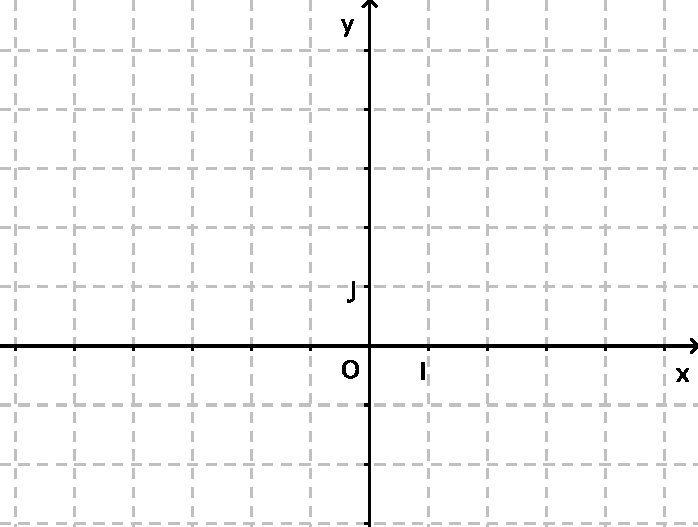
\includegraphics[width=8cm]{F_Axes.pdf}    
\par}

\begin{definition}
  \fbox{
    \begin{minipage}[t]{0.85\linewidth}
      Si une fonction $f$ a pour représentation graphique la courbe
      $\mathscr{C}$, on dit que cette courbe $\mathscr{C}$ \emph{a pour
        équation} $y=f(x)$ dans le repère choisi.
    \end{minipage}
  }
\end{definition}

\begin{example}
    Soit la fonction \( f(x)=3x-1\).
    \begin{enumerate}
        \item
            Le point \( (0,-1)\) est sur la courbe représentative de \( f\) parce que \( f(0)=1\).
        \item
            Le point \( (10,29)\) est également sur la courbe parce que \( f(10)=29\).
        \item
            Le point \( (2,3)\) n'est par contre pas sur le graphe parce que \( f(2)=5\neq 4\).
    \end{enumerate}
\end{example}

\begin{definition}
    Une classe importante de fonctions sont les fonctions de la forme \( f(x)=ax\) où \( a\) est un nombre. Une telle fonction est dite \defe{linéaire}{linéaire (fonction)}. 

    Les fonctions du type \( f(x)=ax+b\) sont des fonctions \defe{affines}{affine (fonction)}. 
\end{definition}
Les fonctions linéaires et affines sont très importantes parce que leur graphe sont des droites. Les fonctions linéaires sont des droites qui passent par l'origine \( (0,0)\) tandis que les fonctions affines (avec \( b\neq 0\)) sont des droites ne passant pas par \( (0,0)\).


\begin{itemize}
\item
    Pour une valeur $x$ sur l'axe des abscisses, il y a un et un seul point d'abscisse $x$ sur la courbe.
\item
    Pour tracer une courbe, il faut placer des points. Plus on choisit de points, plus la courbe sera précise.
\end{itemize}

\begin{rem}
  \begin{minipage}[t]{0.45\linewidth}
    Cette courbe ne représente pas une fonction, car le nombre $x$ a
    deux images $y$.    
  \end{minipage}
  \qquad
  \begin{minipage}[c]{0.4\linewidth}
    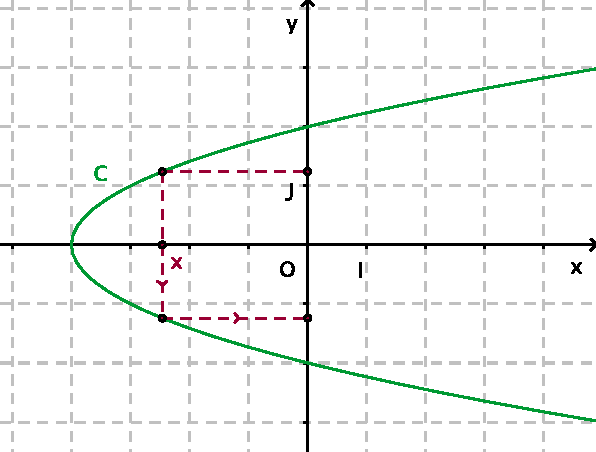
\includegraphics[width=5cm]{F_NonFct.pdf}
  \end{minipage}
\end{rem}


\paragraph{Cas particulier :} 
\begin{minipage}[t]{0.8\linewidth}
  Si $f$ est une fonction affine définie pour $x\in\R$ par 
  $f(x)=ax+b$, et si la droite $d$ est sa représentation graphique,
  une équation de la droite $d$ est \ $y=ax+b$.
\end{minipage}

\paragraph{Application :} 
\begin{minipage}[t]{0.8\linewidth}
  Pour $x\in\R$, $f(x)=-x^2+2x$, de courbe représentative
  $\mathscr{P}$.\\
  Le point $A(2;0)$ appartient-il à $\mathscr{P}$ ? De même pour
  $B(-2;-7)$.
  \vspace{4cm}
\end{minipage}

\section{Résolution graphique d'(in)équations} 

\begin{definition}
    Soit \( f\) une fonction sur \( \eR\). Nous disons que \( a\in \eR\) est un \defe{antécédent}{antécédent} du nombre \( y\) si \( y=f(a)\). Autrement dit, les antécédents de \( a\) sont les éléments de \( \eR\) dont l'image par \( f\) est \( a\).
\end{definition}

\begin{example}
    Le nombre \( 4\) est un antécédent de \( 3\) pour la fonction \( f(x)=\frac{ x }{ 2 }+1\).
\end{example}

\begin{example}
    Les nombres \( 3\) et \( -3\) sont tout deux des antécédents de \( 9\) pour la fonction \( x\mapsto x^2\).
\end{example}

\subsection{Lecture graphique d'images / antécédents}

\begin{minipage}[c]{0.4\linewidth}
  On considère 
  $
  \begin{array}[t]{cl}
    f : & \R \longrightarrow \R \\
    & x \longmapsto x^2
  \end{array}
  $.  \\

  A $x$, on associe $y=f(x)$. 

  \vspace{1cm}

  \begin{itemize}
  \item[\textbullet] Image de $1,5$ ? \\[2em]
  \item[\textbullet] Antécédent de $3,5$ ?  \\[2em]
  \item[\textbullet] Antécédent de $-1$ ? \\[2em]
  \item[\textbullet] Antécédent de $0$ ?  \\[2em]
  \end{itemize}
  
\end{minipage}
\begin{minipage}[c]{0.6\linewidth}
  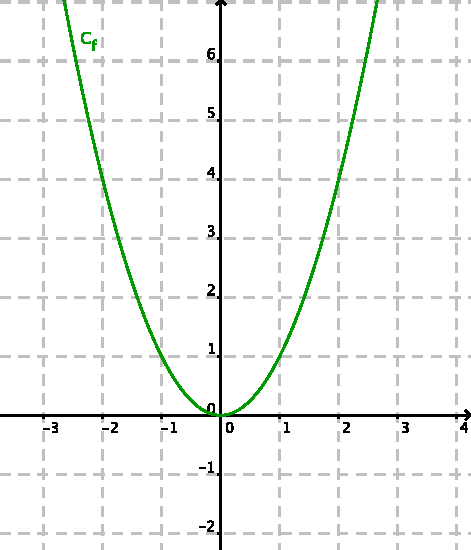
\includegraphics[width=9cm]{F_Carre2.pdf}  
\end{minipage} \\


Fonction $f(x)=x^2$ \\[2ex]
\begin{tabular}{|>{$}c<{$}|*{11}{>{\centering$}p{1cm}<{$}|}c}
  \cline{1-12}
  \displaystyle \vphantom{\int} \ x \ \ 
  & -4 & -3 & -2 & -1 & 0 & 1 & 2 & 3 & 4 & -0,5 & 0,5 & \\
  \cline{1-12}
  \displaystyle \vphantom{\int} y
  & & & & & & & & & & & \\
  \cline{1-12}
\end{tabular}

\medskip


\subsection{Résolution graphique d'équations}

$k$ est un réel fixé. \\

\noindent
\fbox{
  \textbullet \quad
  Résoudre l'équation $f(x)=k$ revient à chercher les antécédents par
  $f$ du nombre $k$.
} \\

Le nombre de solutions de l'équation $f(x)=k$ est égal au nombre de
points d'intersection de la courbe $\mathscr{C}$ avec la droite $d$
d'équation $y=k$. Les solutions sont les abscisses de ces points
d'intersection. 

\paragraph{Exemple :} 
\begin{minipage}[t]{0.55\linewidth}
  On cherche à résoudre $f(x)=4$. \\
  On trace la droite d'équation \hspace{1.5cm} et
  on observe les points d'intersection de cette droite avec la courbe
  $\mathscr{C}$. \\[1ex]
  $\mathscr{S}=\{\hspace{1.5cm}\}$. 
\end{minipage}
\qquad
\begin{minipage}[c]{0.25\linewidth}
  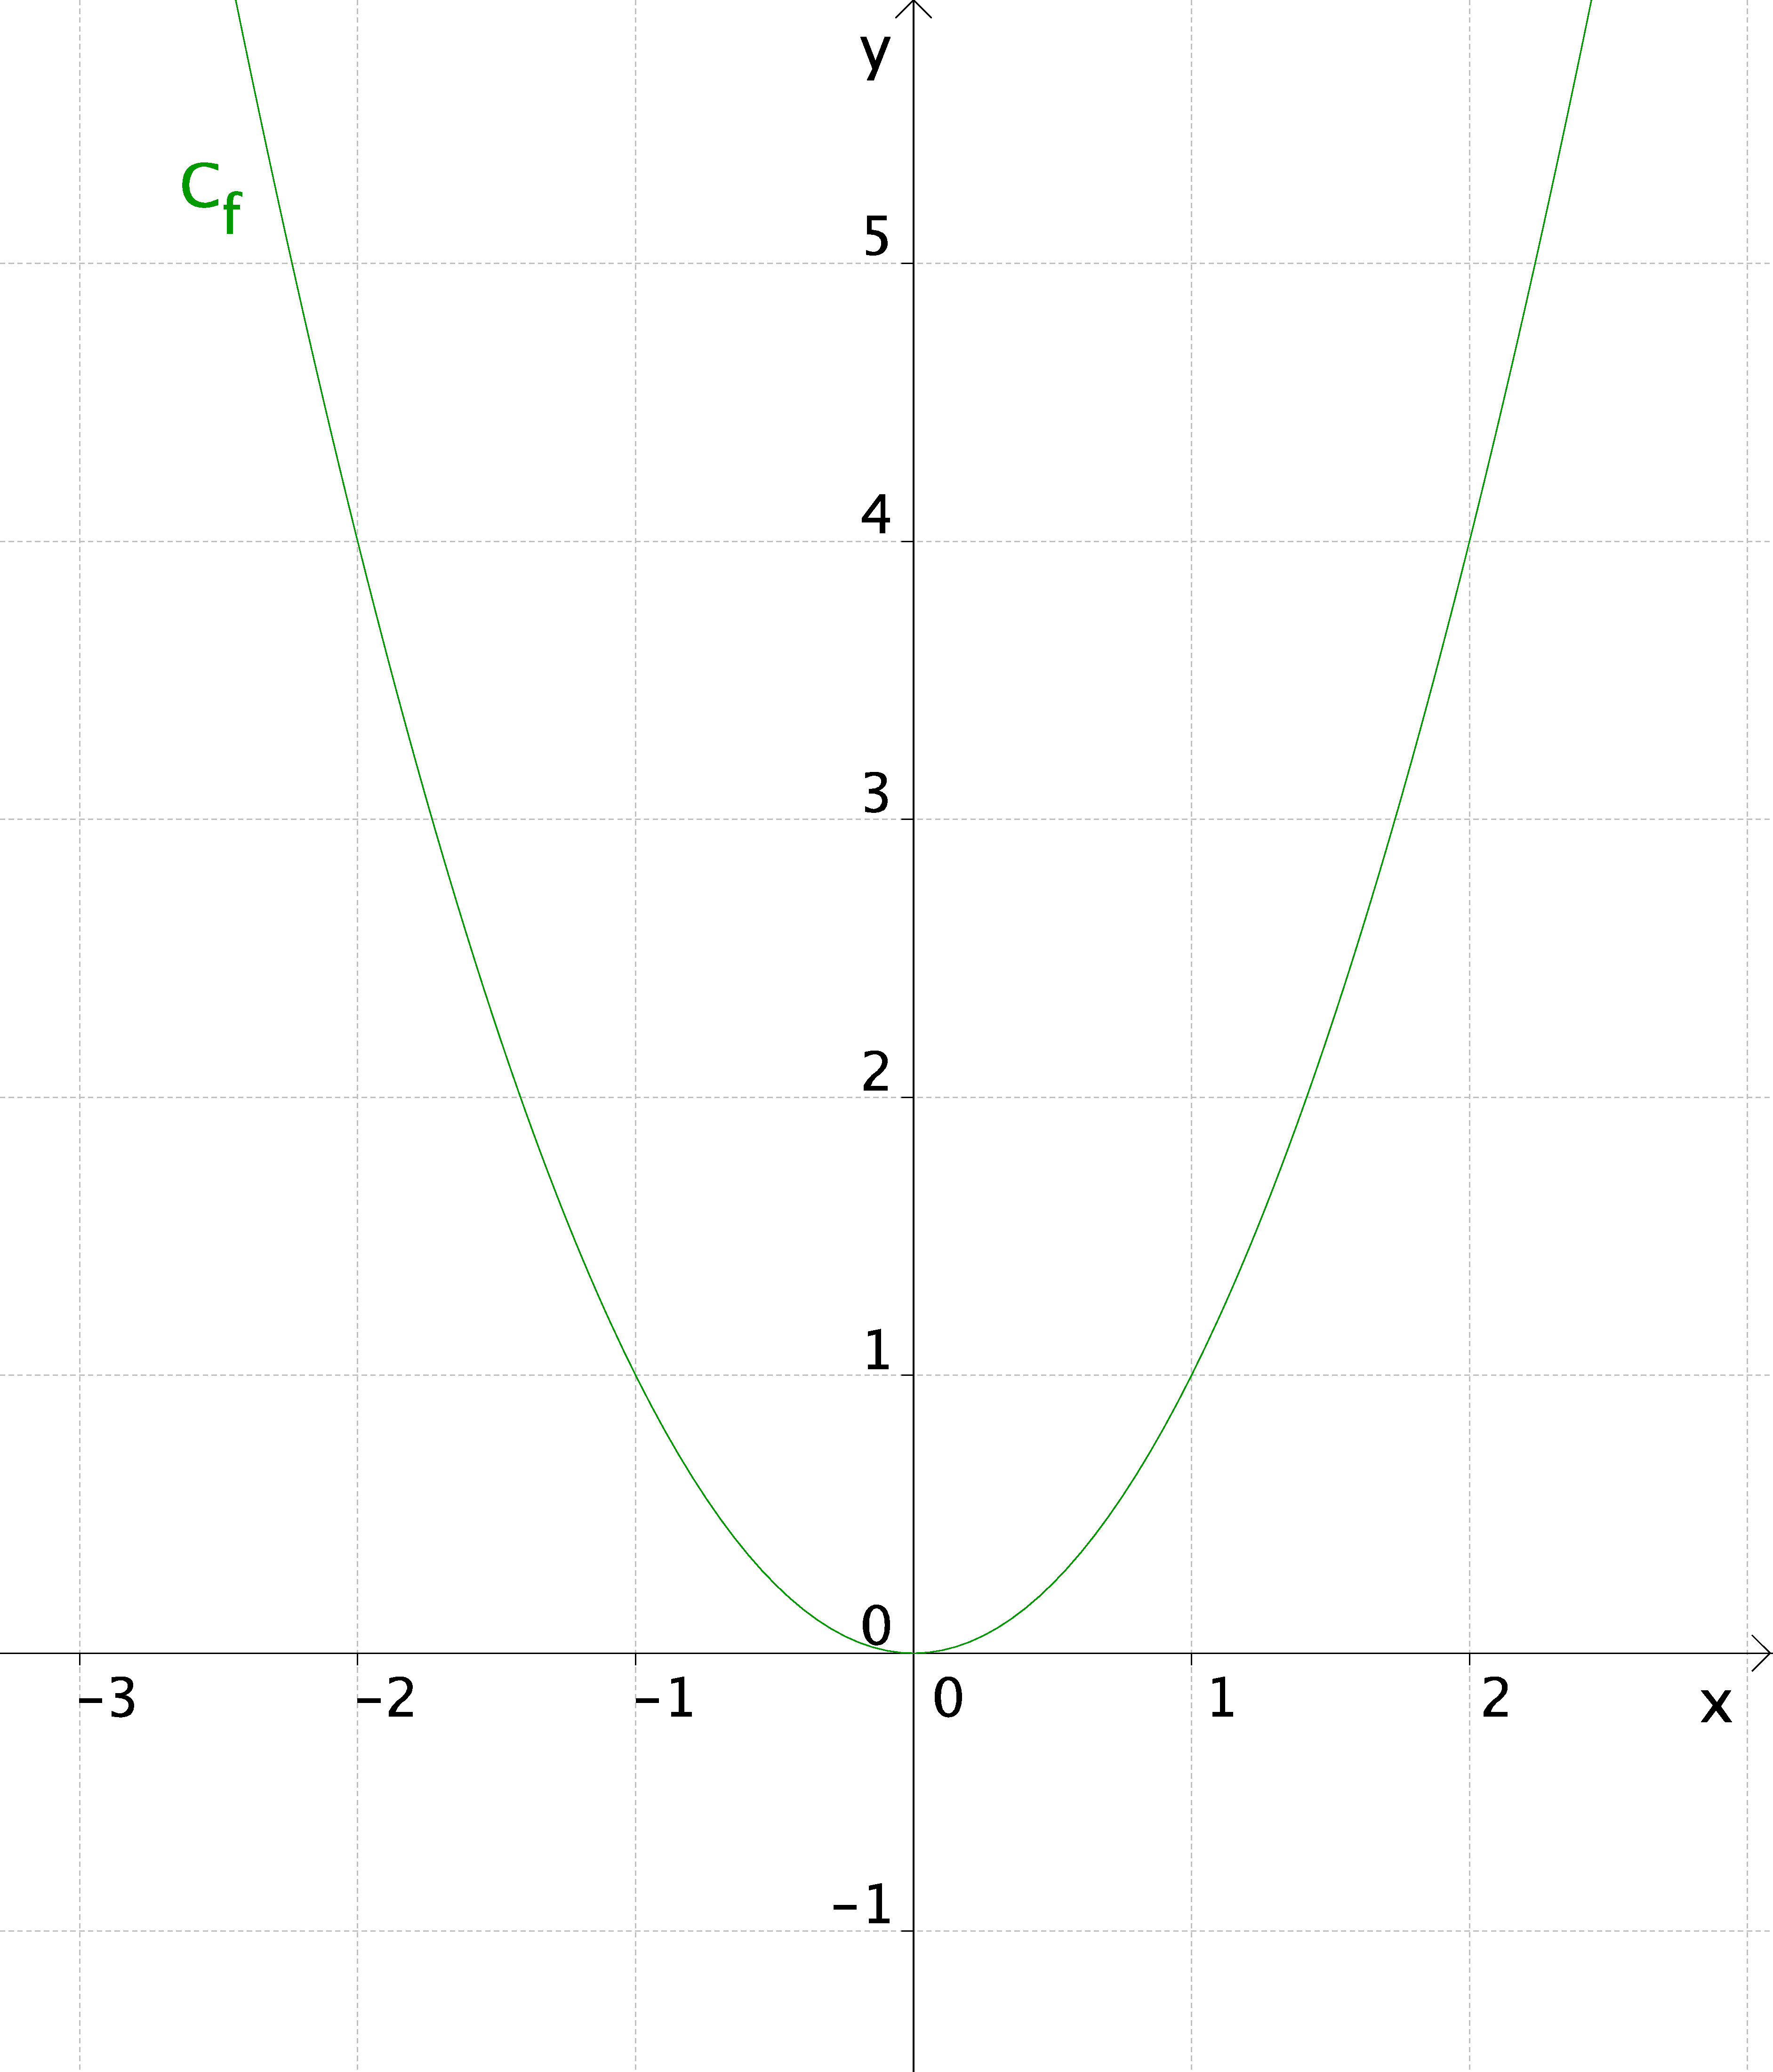
\includegraphics[width=\textwidth]{F_reseq_f.pdf}
\end{minipage}

\pagebreak[4]

\noindent
\fbox{
  \begin{minipage}[t]{1.0\linewidth}
    \textbullet \quad 
    Résoudre l'équation $f(x)=g(x)$ revient à déterminer les abscisses
    des points d'intersection des courbes $\mathscr{C}_f$ et
    $\mathscr{C}_g$.
  \end{minipage}
} \\[1em]

\begin{minipage}[c]{0.5\linewidth}
  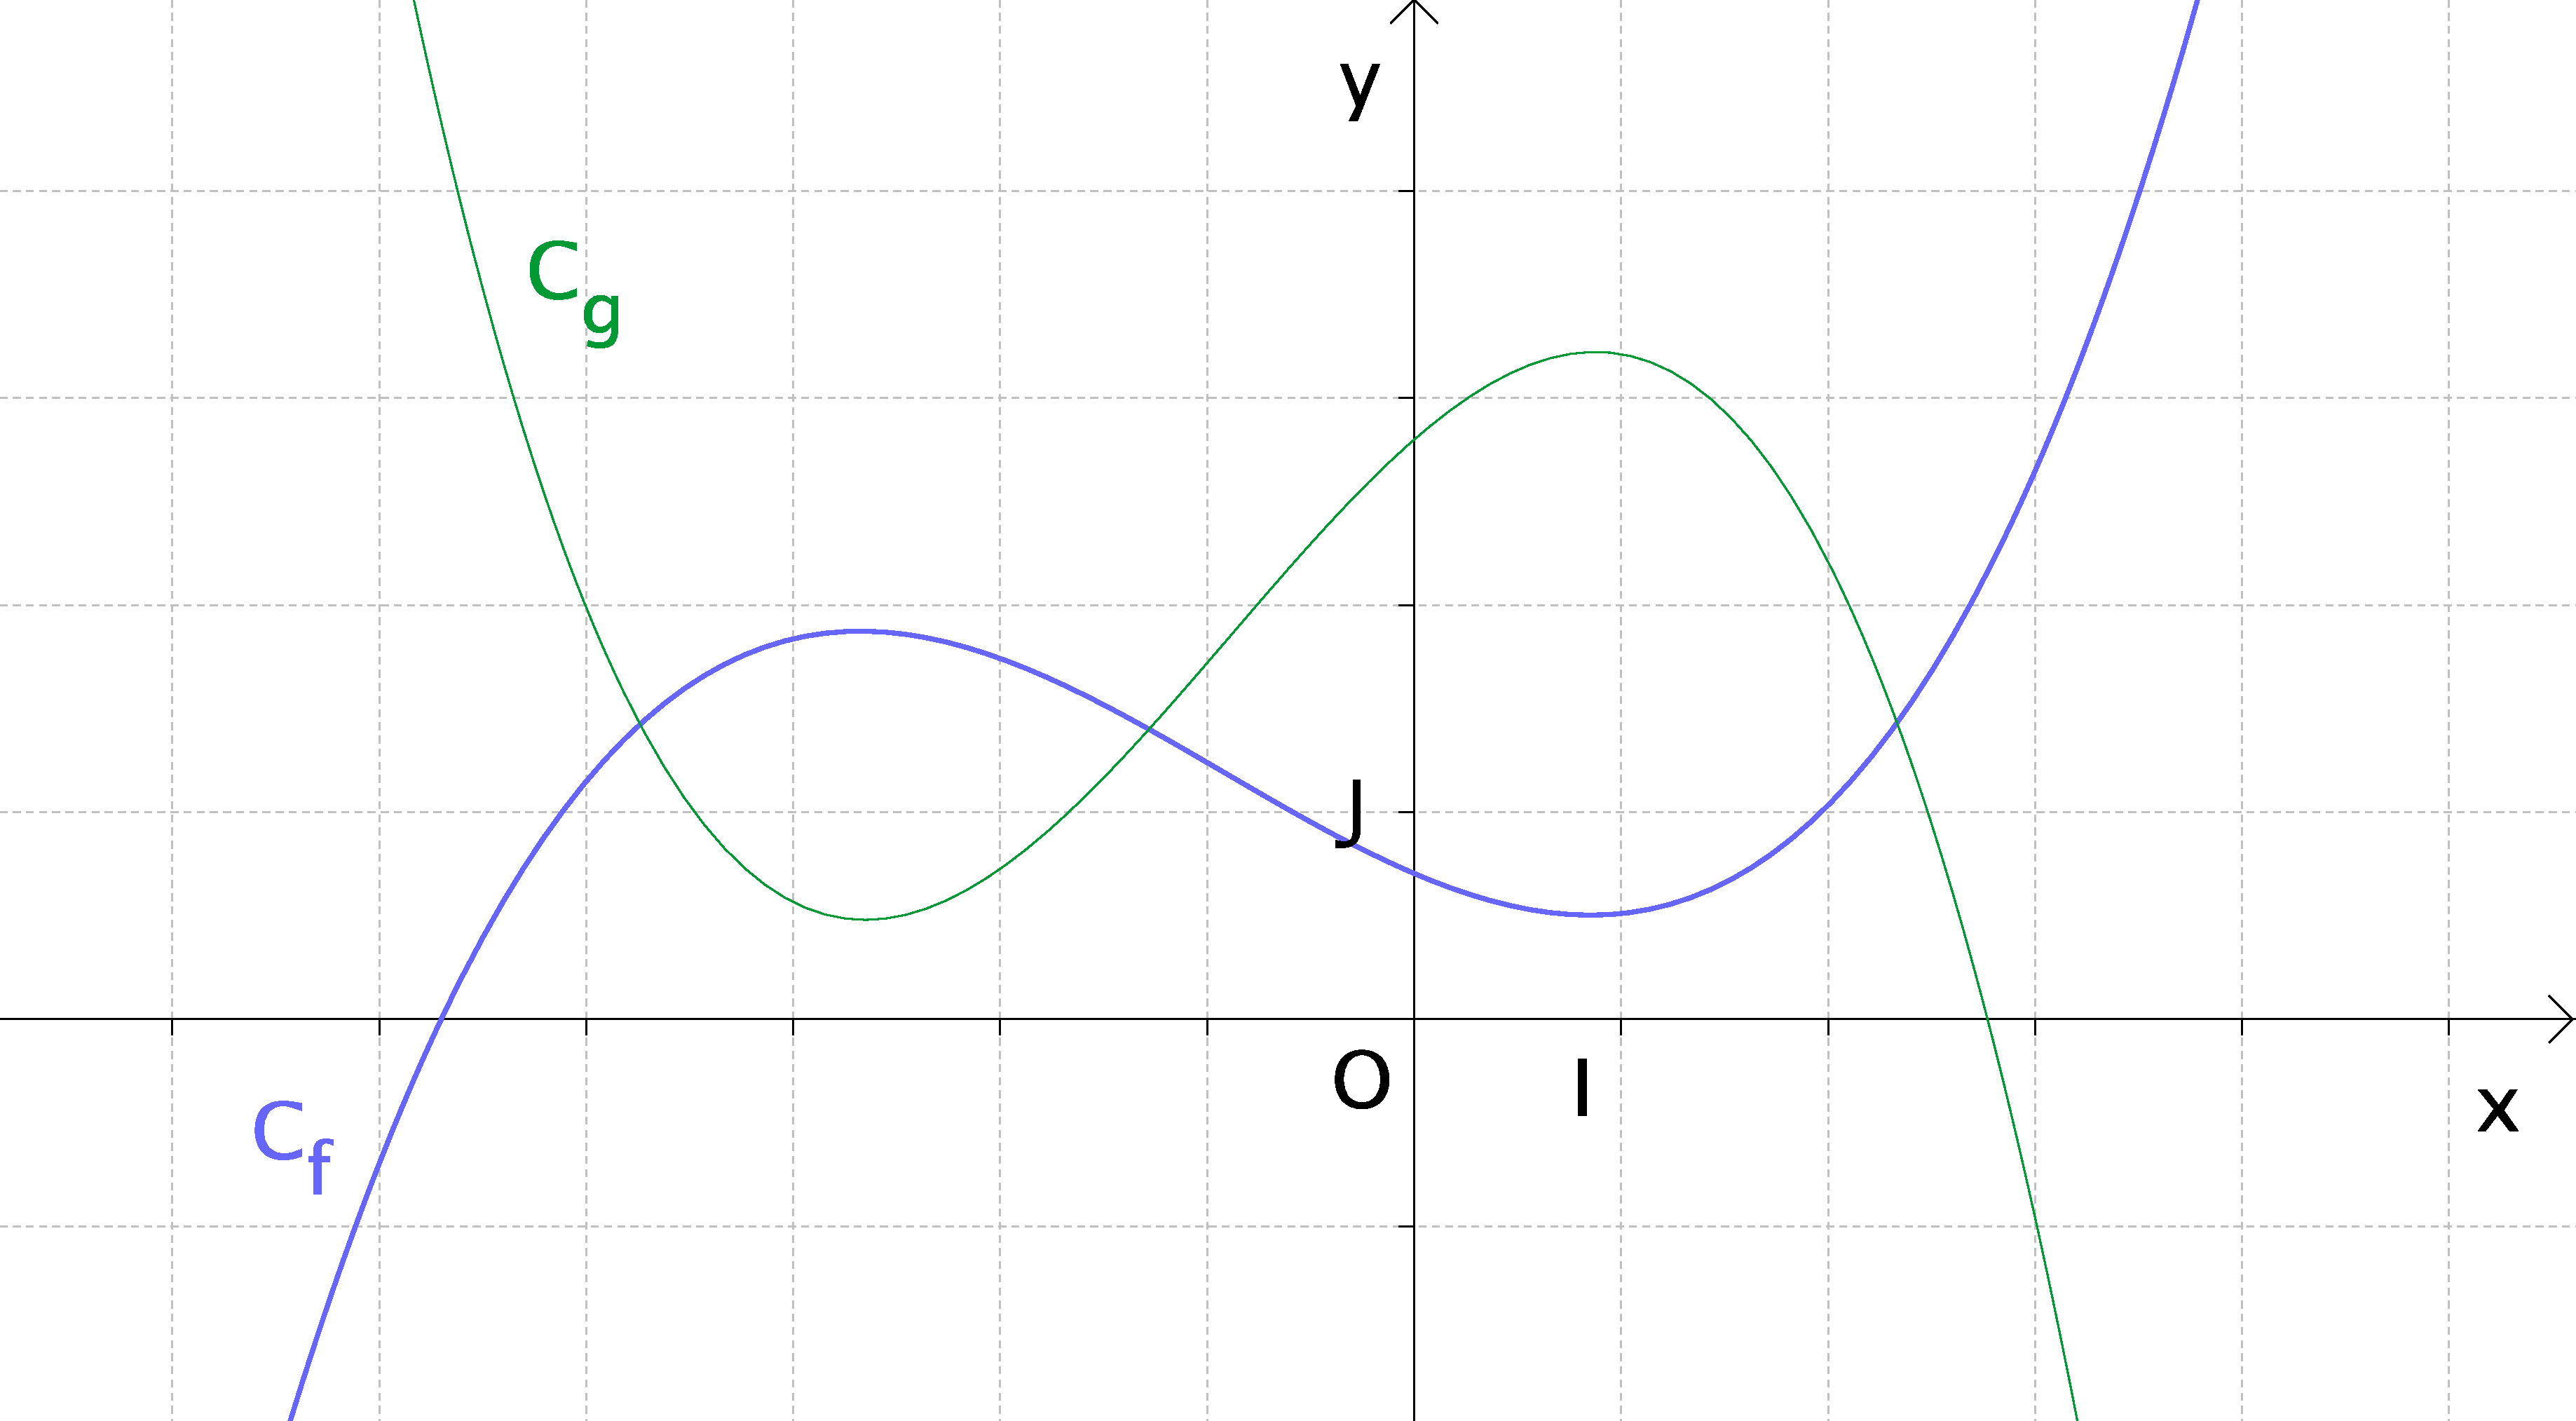
\includegraphics[width=\textwidth]{F_resineq_fg.pdf}
\end{minipage}
\qquad
\begin{minipage}[t]{0.4\linewidth}
  Sur cette figure, l'équation $f(x)=g(x)$ a \hspace{1cm} solutions,
  qui sont
\end{minipage} \\[1em]



\subsection{Résolution graphique d'inéquations}

\paragraph{\textbullet \ Inéquation du type $f(x)<k$} \ \par
Les solutions de l'inéquation $f(x)<k$ sont les abscisses des points
de $\mathscr{C}$ situés en-dessous de la droite d'équation $y=k$.

En particulier, les solutions de l'inéquation $f(x)<0$ sont les
abscisses des points de la courbe $\mathscr{C}$ qui sont situés
en-dessous de l'axe des abscisses, c'est-à-dire ayant une ordonnée
strictement négative.\\

\medskip

{\centering
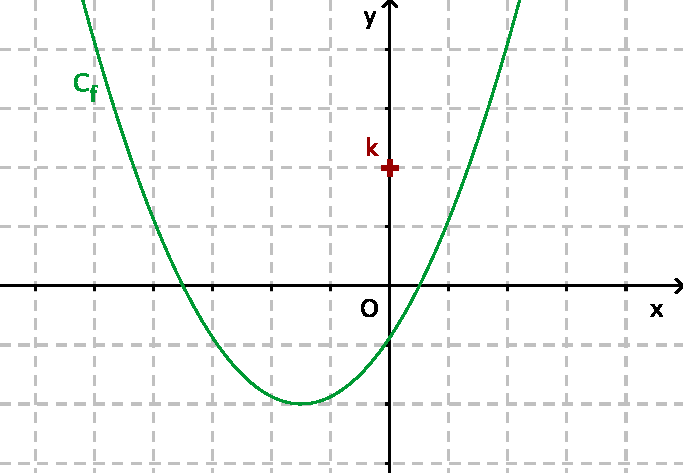
\includegraphics[width=0.5\textwidth]{F_resineq_f.pdf}
\par}

\medskip

On procède de la même manière pour les inégalités du type $f(x)>k$,
$f(x)\geq k$, $f(x)\leq k$. 

\paragraph{\textbullet \ Inéquation du type $f(x)<g(x)$} \ \par
Les solutions de l'inéquation $f(x)<g(x)$ sont les abscisses des
points pour lesquels la courb $\mathscr{C}_f$ et en-dessous de la
courbe $\mathscr{C}_g$.

\medskip

{\centering
  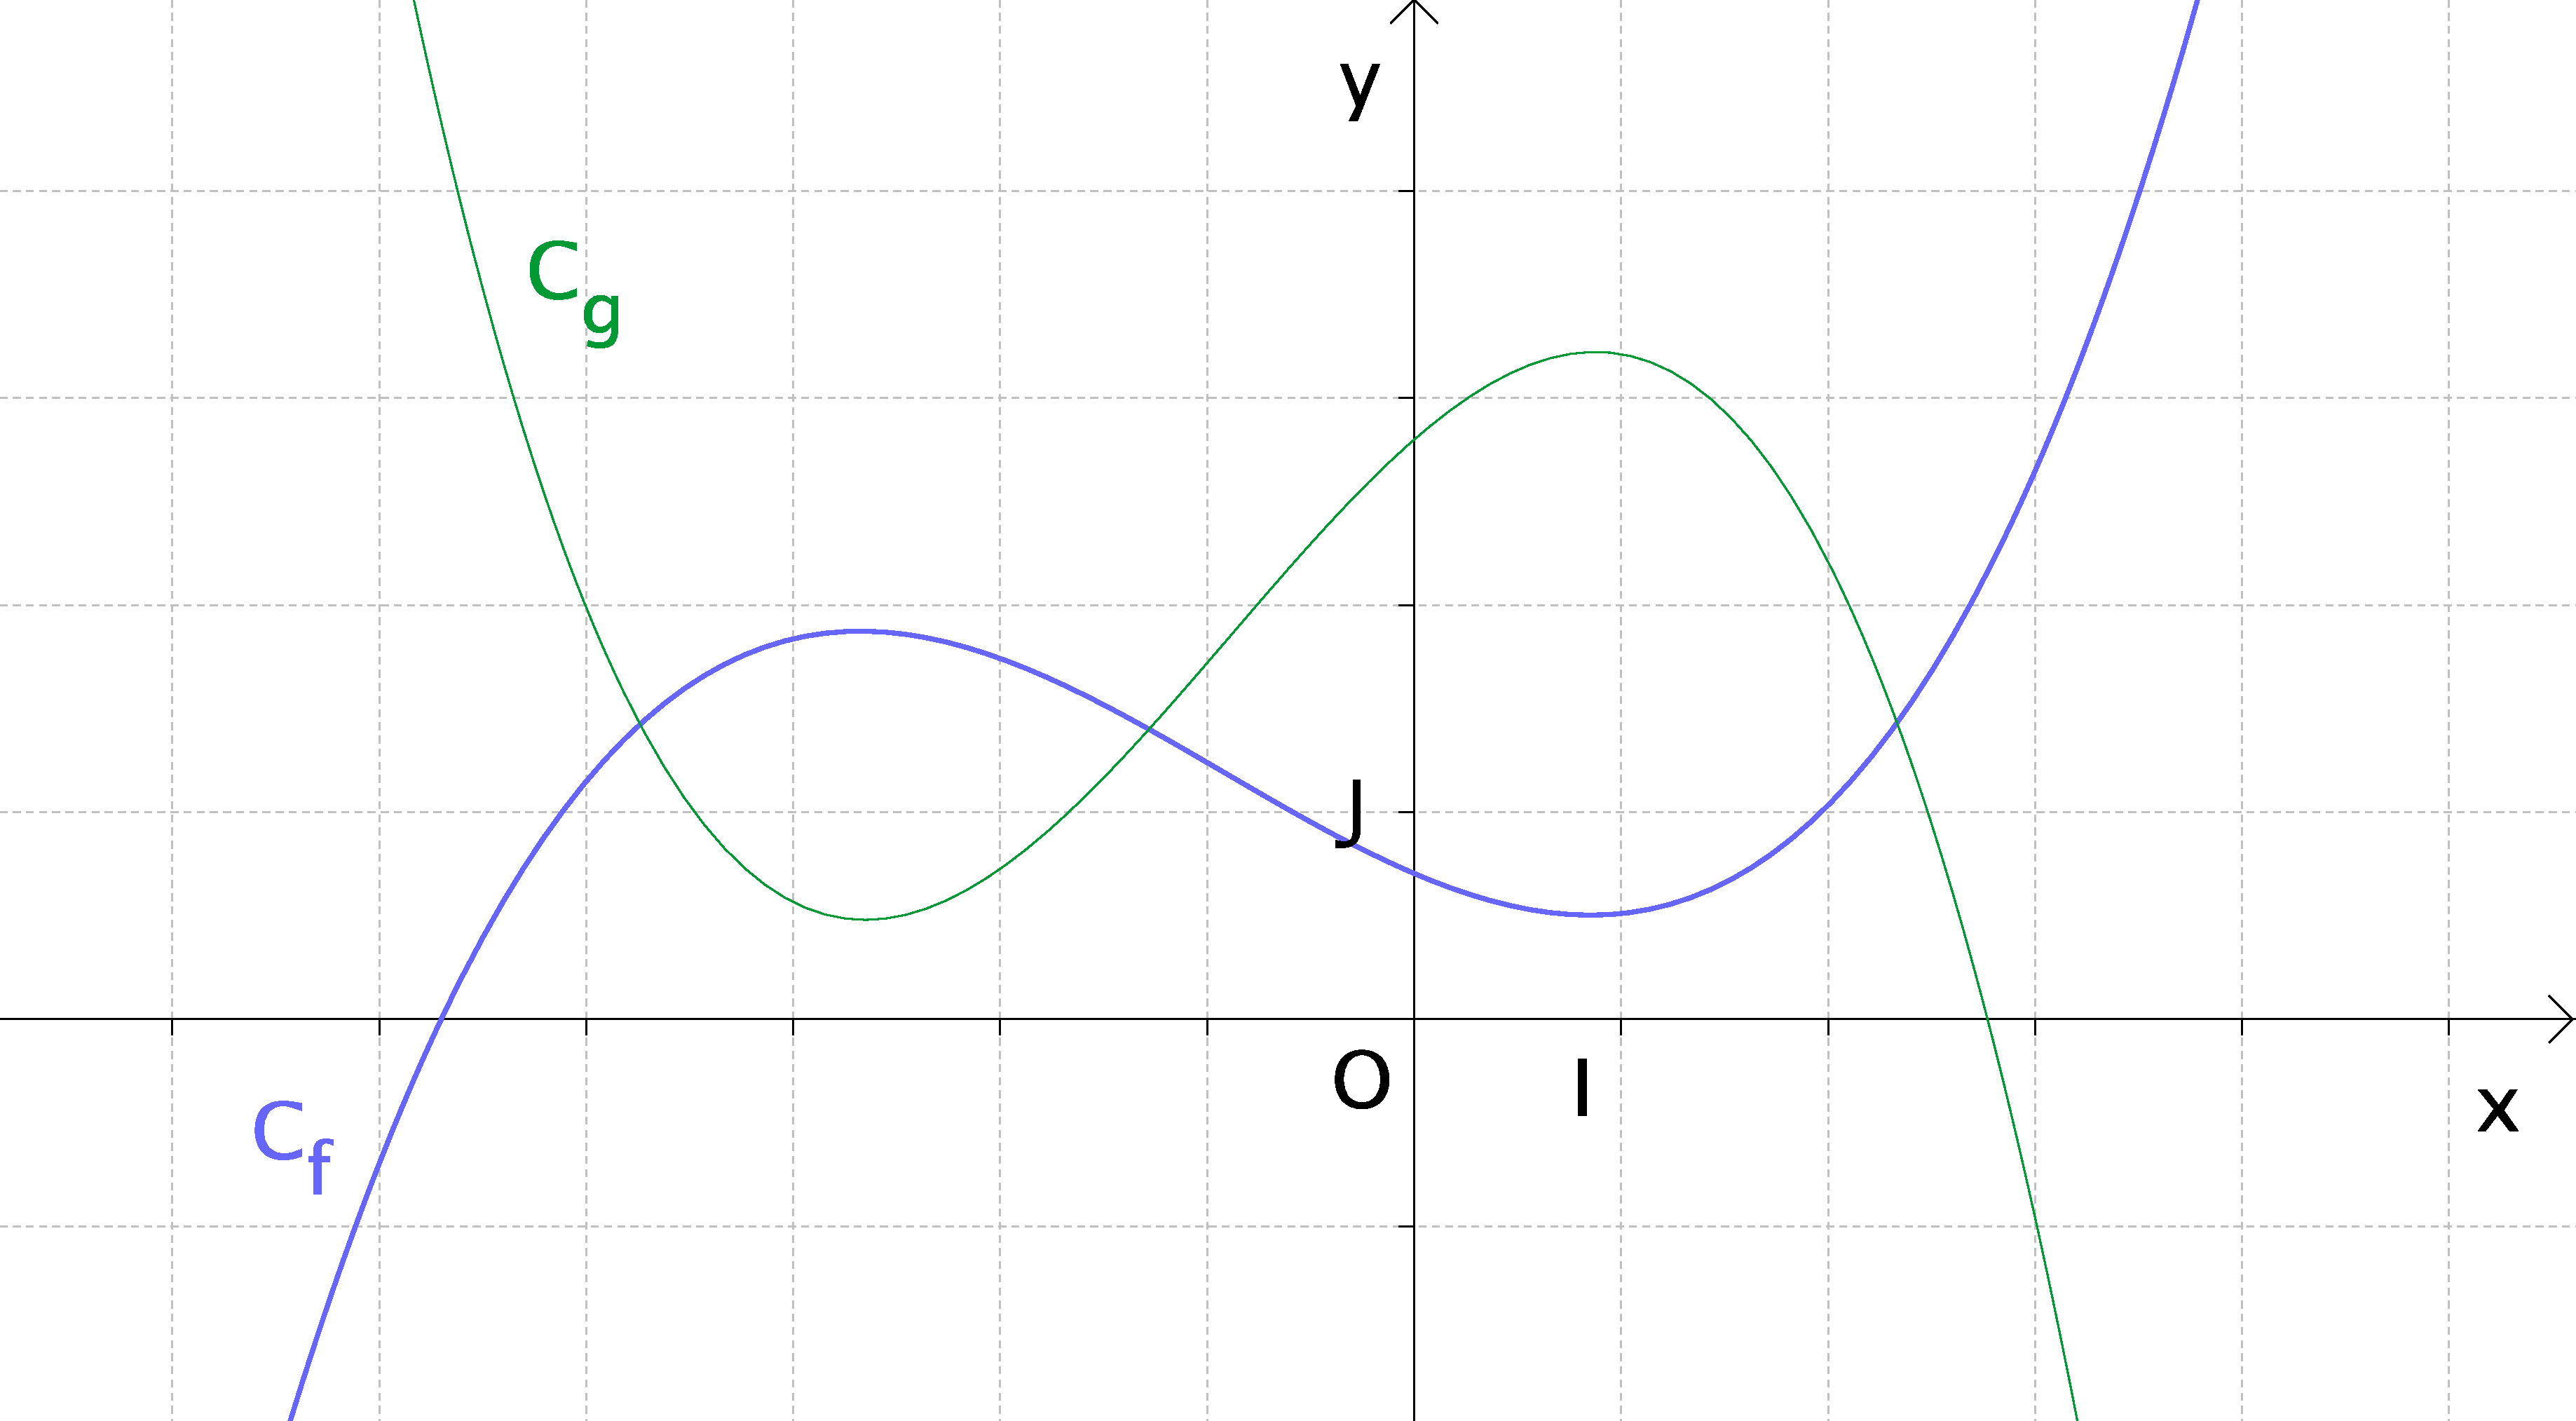
\includegraphics[width=0.5\textwidth]{F_resineq_fg.pdf}
\par}

%\clearpage


\section{Sens de variation d'une fonction}
\label{sec:variations}

\subsection{Notion intuitive}
\label{ssec:notion_intuitive}

\vspace{2cm}

\begin{center}
  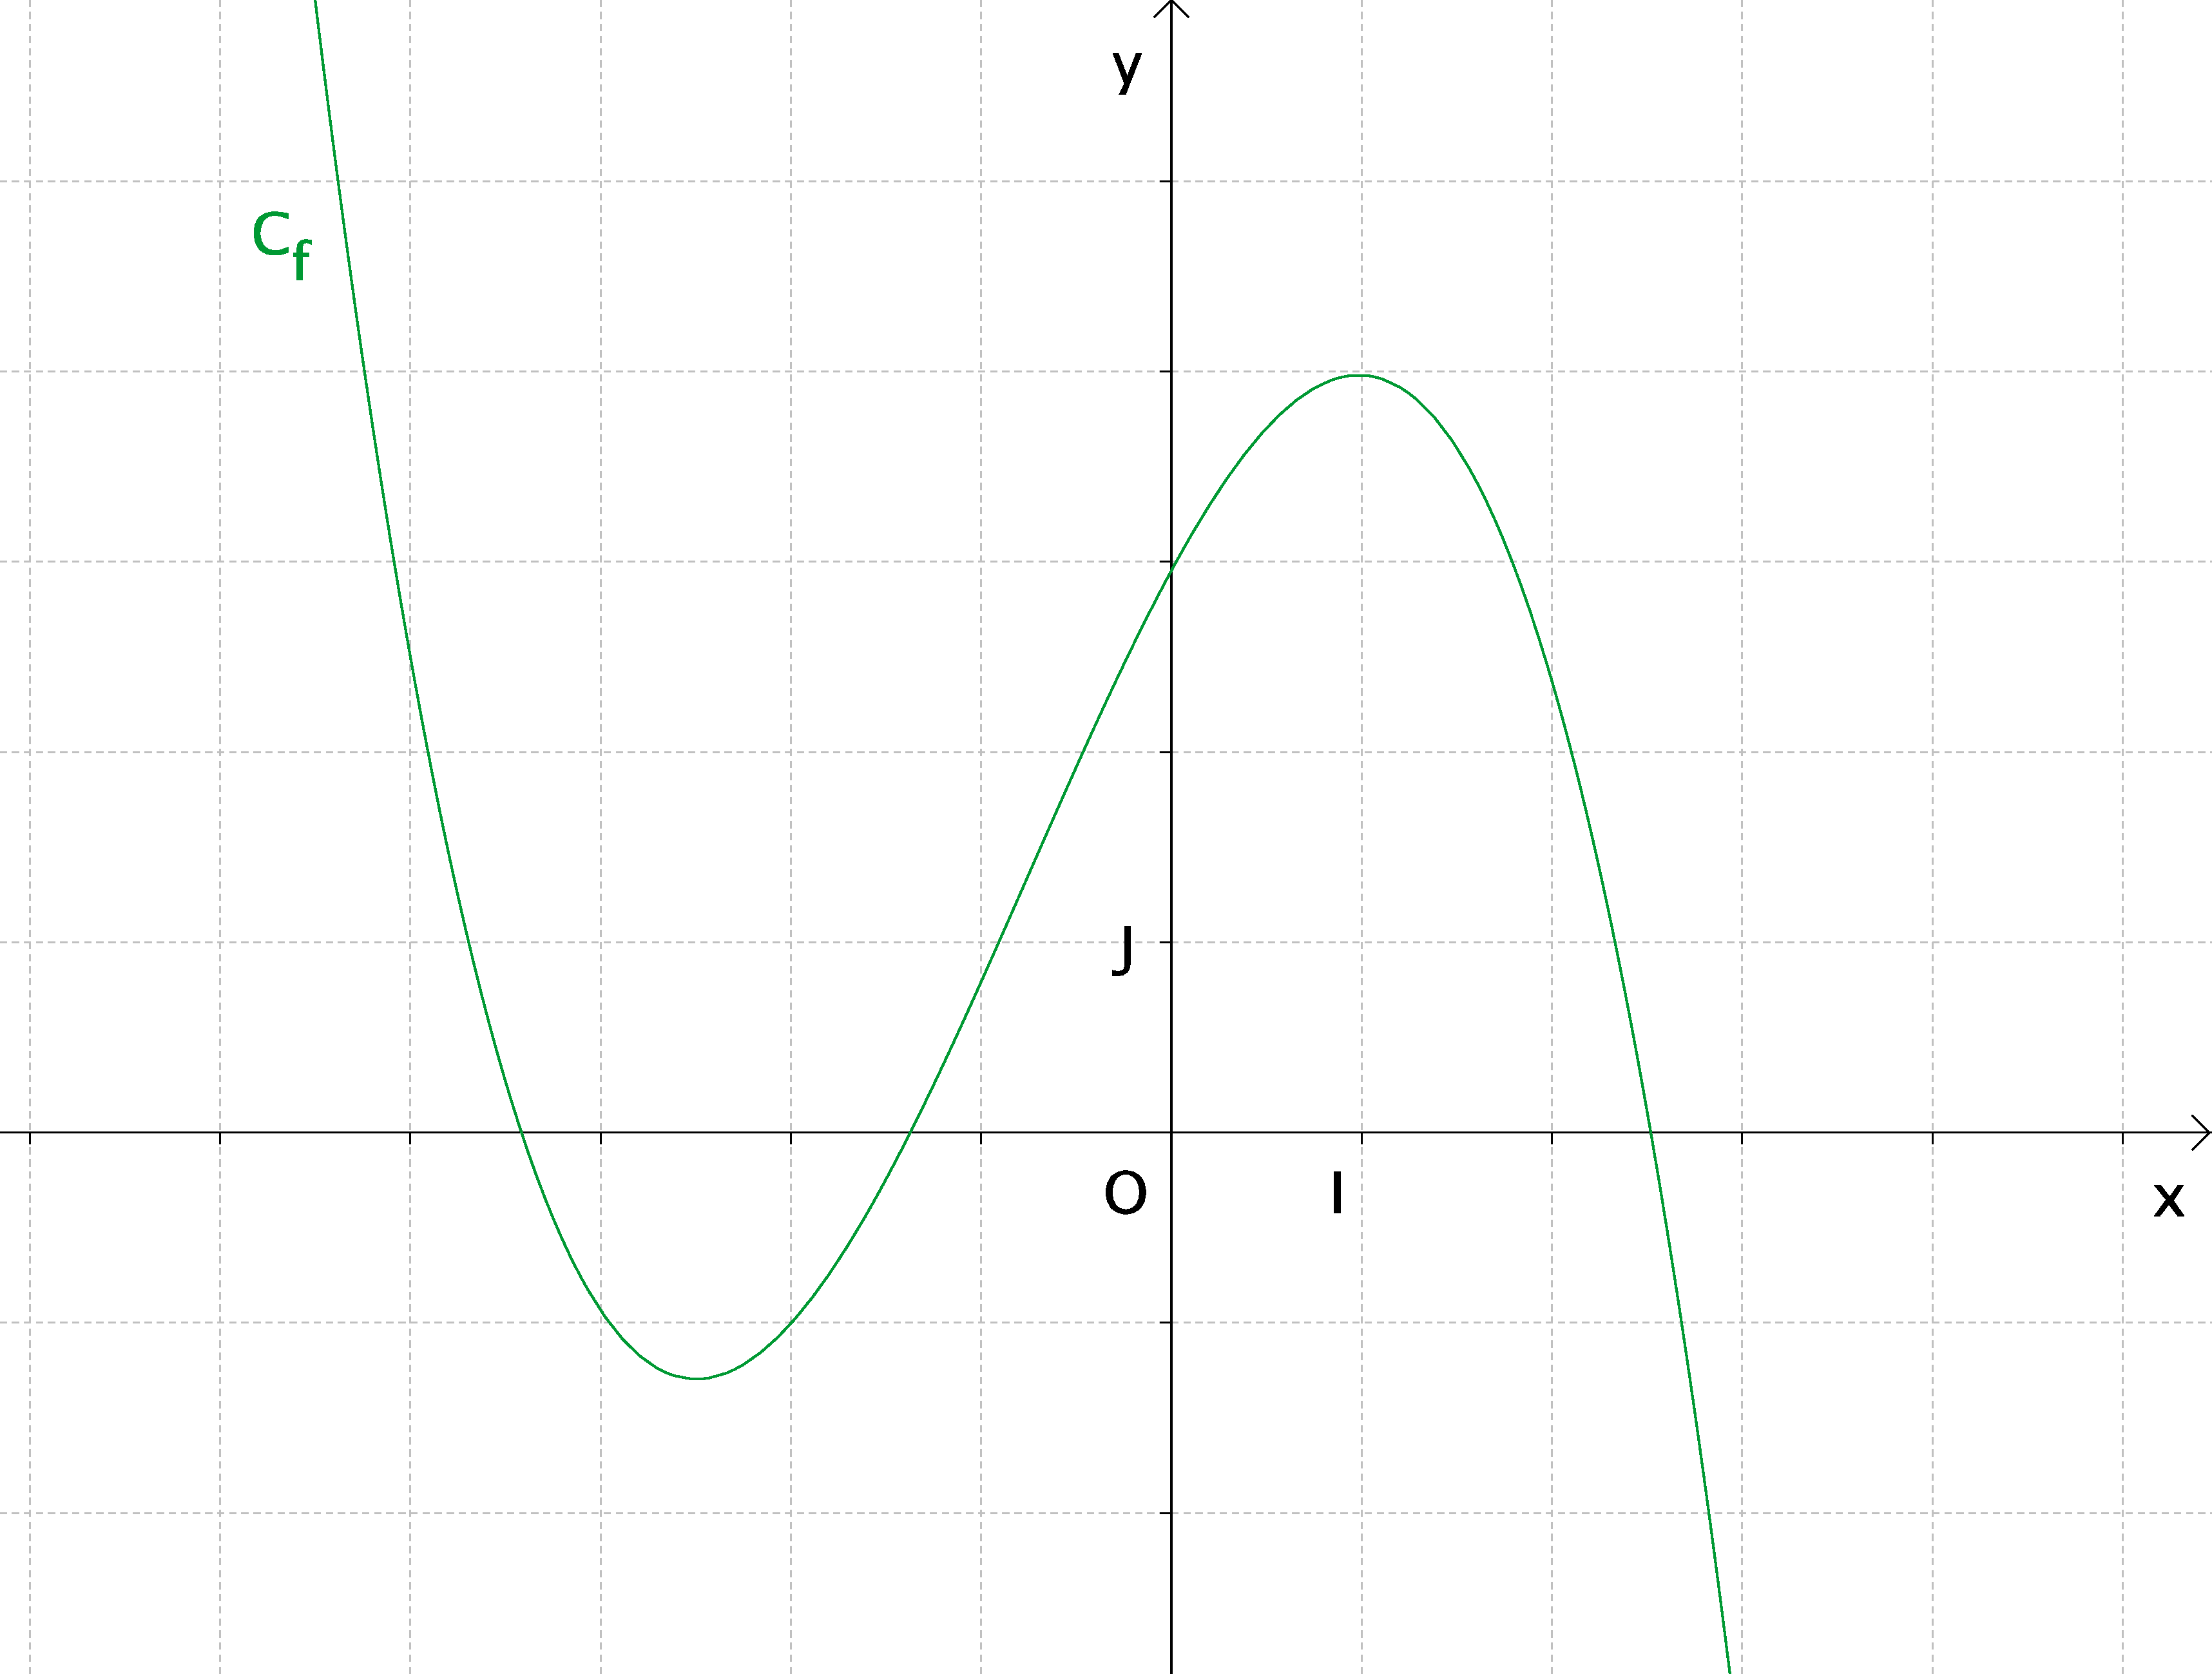
\includegraphics[width=0.6\textwidth]{F_Variations.pdf}
\end{center}

\vspace{2cm}



\subsection{Définition}

\begin{definition}
  \fbox{
    \begin{minipage}[t]{0.82\linewidth}
      Soit $f$ une fonction définie sur $\defD$ et $I$ un
      intervalle de $\defD$.\\[-2ex]
      \begin{itemize}
      \item[\textbullet] On dit que $f$ est \emph{croissante} sur $I$
        si et seulement si pour tous réels $a$ et $b$ de $I$, \\
        \ \quad si $a\leq b$ \ alors \ $f(a)\leq f(b)$.\\[-2ex]
      \item[\textbullet] On dit que $f$ est \emph{décroissante} sur $I$
        si et seulement si pour tous réels $a$ et $b$ de $I$, \\
        \ \quad si $a\leq b$ \ alors \ $f(a)\geq f(b)$. 
      \end{itemize}
    \end{minipage}
  }
\end{definition}

\smallskip

\begin{rem}
  \begin{minipage}[t]{0.8\linewidth}
    Une fonction croissante range les images dans le même ordre que
    les antécédents. \\
    Une fonction décroissante inverse cet ordre. \\
  \end{minipage}
\end{rem}

\begin{center}
  \begin{tabular}{c@{\qquad \qquad}c}
    \begin{minipage}[c]{0.36\linewidth}
      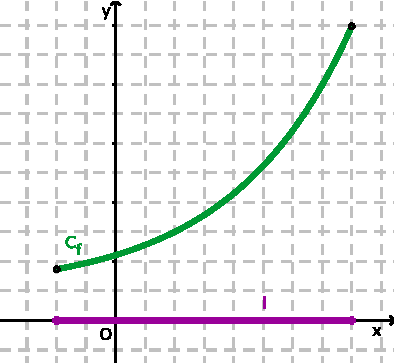
\includegraphics[width=\textwidth]{F_Croissante.pdf}
    \end{minipage}
    &
    \begin{minipage}[c]{0.36\linewidth}
      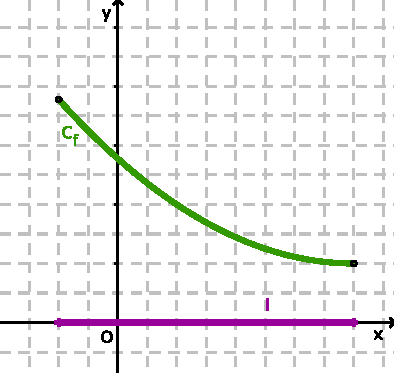
\includegraphics[width=\textwidth]{F_Decroissante.pdf}
    \end{minipage}  \\
    & \\
    $f$ croissante sur $I$
    &
    $f$ décroissante sur $I$
  \end{tabular}
\end{center}


\begin{rem}
  \begin{minipage}[t]{0.84\linewidth}
  On dit que $f$ est \emph{\underline{strictement} croissante}
  (respectivement \emph{\underline{strictement} décroissante}) sur~$I$
  si pour tous réels $a$ et $b$ de $I$ tels que $a<b$, on a
  $f(a)<f(b)$ (respectivement $f(a)>f(b)$).  \\
  \end{minipage}
\end{rem}

\begin{rem}
  \begin{minipage}[t]{0.8\linewidth}
    Dans cette définition, il est important que $I$ soit un
    intervalle. \\ $]-\infty;0[\ \cup \ ]0;+\infty[$ n'est pas un
    intervalle. \\
  \end{minipage}
\end{rem}

\begin{definition}
  \fbox{
    \begin{minipage}[t]{0.82\linewidth}
      On appelle fonction \emph{monotone} sur $I$ une fonction qui est
      soit croissante sur $I$, soit décroissante sur $I$.
    \end{minipage}
  }
\end{definition}

\smallskip

La fonction représentée en \,IV.\,1) n'est pas
monotone sur $[-4;3]$. Elle est monotone sur $[-4;-2,5]$
(décroissante), sur $[-2,5;1]$ (croissante), et sur $[1;3]$ (décroissante).\\

\begin{definition}
  \fbox{
    \begin{minipage}[t]{0.82\linewidth}
      On dit que $f$ est \emph{constante} sur $I$ lorsque pour tous
      les réels $a$ et $b$ de $I$, on a $f(a)=f(b)$. (Tous les réels de
      $I$ ont la même image par $f$).
    \end{minipage}
  }
\end{definition}

\begin{minipage}[t]{0.4\linewidth}
  Dans ce cas, il existe $k\in\R$ tel que \\ pour tout $a\in I$, $f(a)=k$.
\end{minipage}
\qquad
\begin{minipage}[c]{0.4\linewidth}
  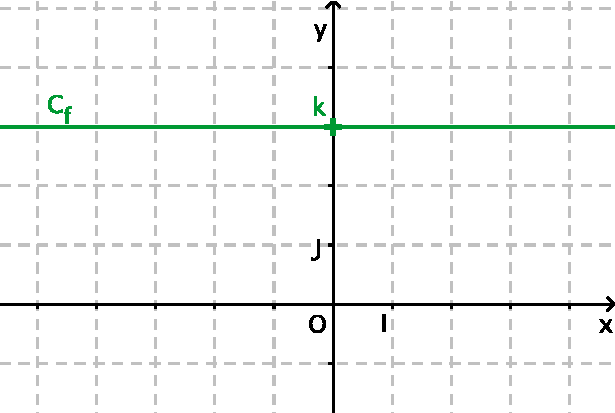
\includegraphics[width=\textwidth]{F_Constante.pdf}
\end{minipage}



\subsection{Tableau de variations}

\og Étudier les variations de $f$ \fg{} signifie {\ldots}


Ces résultats sont résumés dans un tableau de variations. \\

%\begin{center}
  %\begin{minipage}[c]{0.4\linewidth}
    %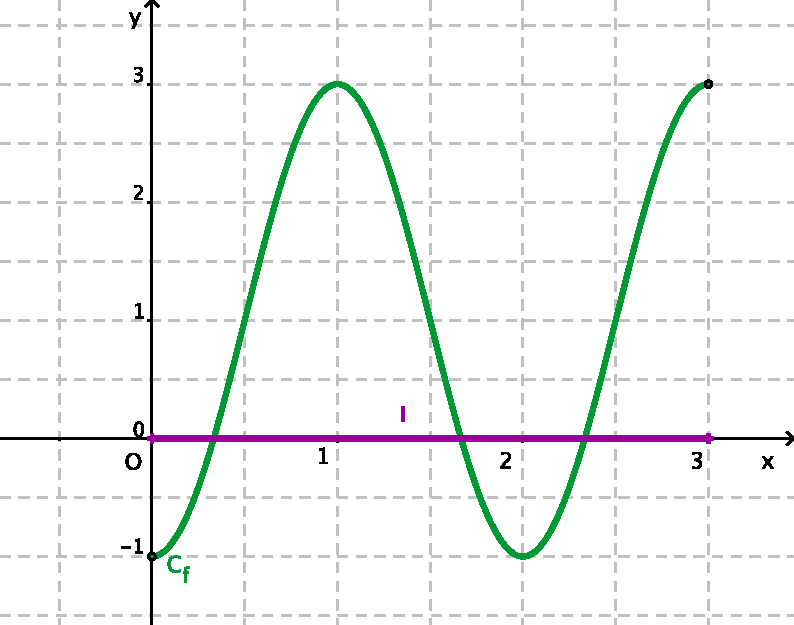
\includegraphics[width=\textwidth]{F_TabVar.pdf}
  %\end{minipage}
  %\qquad \qquad
  %\begin{minipage}[c]{0.5\linewidth}
    %\centering
    %\begin{variations}
      %x & & 0 & & 1 & & 3 & & 4  \; \\
      %\filet
      %\m f & \; & -1 & \c & \h3 & \d & -1 & \c & \h3 \\
    %\end{variations}        
  %\end{minipage} \\[1em]
  %\begin{minipage}[c]{0.4\linewidth}
    %\centering
    %$f$ définie sur $[0;4]$
  %\end{minipage}
  %\qquad \qquad
  %\begin{minipage}[c]{0.5\linewidth}
    %\centering
    %$f$ est croissante sur $[0;1]$ et sur $[3;4]$. \\
    %$f$ est décroissante sur $[1;3]$
  %\end{minipage} 
%\end{center}

%TODO : refaire le tableau de variations.

\subsection{Sens de variation d'une fonction affine}

\begin{proposition}
  \fbox{
    \begin{minipage}[t]{0.7\linewidth}
      Soit $f$ la fonction affine $x\mapsto ax+b$.
      \begin{itemize}
      \item[\textbullet] Si $a>0$, alors $f$ est croissante sur $\R$.
      \item[\textbullet] Si $a<0$, alors $f$ est décroissante sur $\R$.
      \item[\textbullet] Si $a=0$, alors $f$ est constante sur $\R$
        (et $f(x)=b$ pour tout $x\in\R$).
      \end{itemize}
    \end{minipage}
  }  
\end{proposition}

\paragraph{Démonstration :} \ \\

\vspace{6cm}


\begin{rem}
  $f(x)=0$ pour $x=\hspace{1cm}$. On connaît donc le signe de $f(x)$
  selon les valeurs de $x$.
\end{rem}


\begin{minipage}[c]{0.4\linewidth}
  \centering
  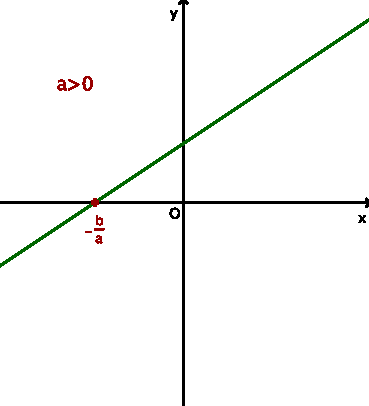
\includegraphics[width=0.6\linewidth]{F_Affine_a.pdf}
\end{minipage}
\quad
\begin{minipage}[c]{0.4\linewidth}
  \centering
  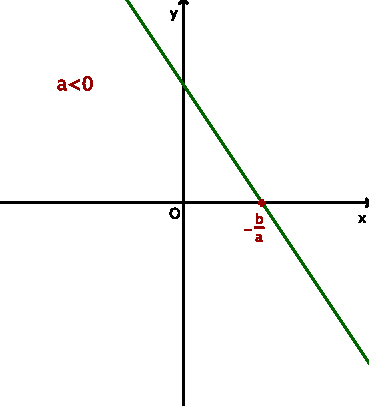
\includegraphics[width=0.6\linewidth]{F_Affine_b.pdf}
\end{minipage}



\begin{proposition}
  \fbox{
    \begin{minipage}[t]{0.85\linewidth}
      Règle du signe de $ax+b$ \\
      
      \begin{tabular}{cc}
        $a<0$ & $a>0$ \\
        & \\
        $\begin{array}{|c|ccccc|}
          \hline
          x & -\infty & & -\dfrac{b}{a} & & +\infty \\[2ex]
          \hline
          ax+b & & + \quad \ & 0 & \quad - & \\[1ex]
          \hline
        \end{array}$
        &
        $\begin{array}{|c|ccccc|}
          \hline
          x & -\infty & & -\dfrac{b}{a} & & +\infty \\[2ex]
          \hline
          ax+b & & - \quad \ & 0 & \quad + & \\[1ex]
          \hline
        \end{array}$ \\
      \end{tabular}  \\[1ex] 
    \end{minipage} \\
  }    
\end{proposition}


\section{Minimum et maximum}

\begin{definition}
  \fbox{
    \begin{minipage}[t]{0.8\linewidth}
      Soit $f$ une fonction définie sur un intervalle $I$. \\[-2ex] 
      \begin{itemize}
      \item[\textbullet] On dit que $f$ admet le réel $m$ pour minimum
        sur $I$ ssi il existe $c\in I$ tel que $f(c)=m$
        et pour tout $x\in I$, $f(x)\geq m$. \\[-2ex]
      \item[\textbullet] On dit que $f$ admet le réel $M$ pour maximum
        sur $I$ ssi il existe $d\in I$ tel que $f(d)=M$ et pour tout
        $x\in I$, $f(x)\leq M$.
      \end{itemize}
    \end{minipage}
  }    
\end{definition}


\begin{minipage}[c]{0.4\linewidth}
  \centering
  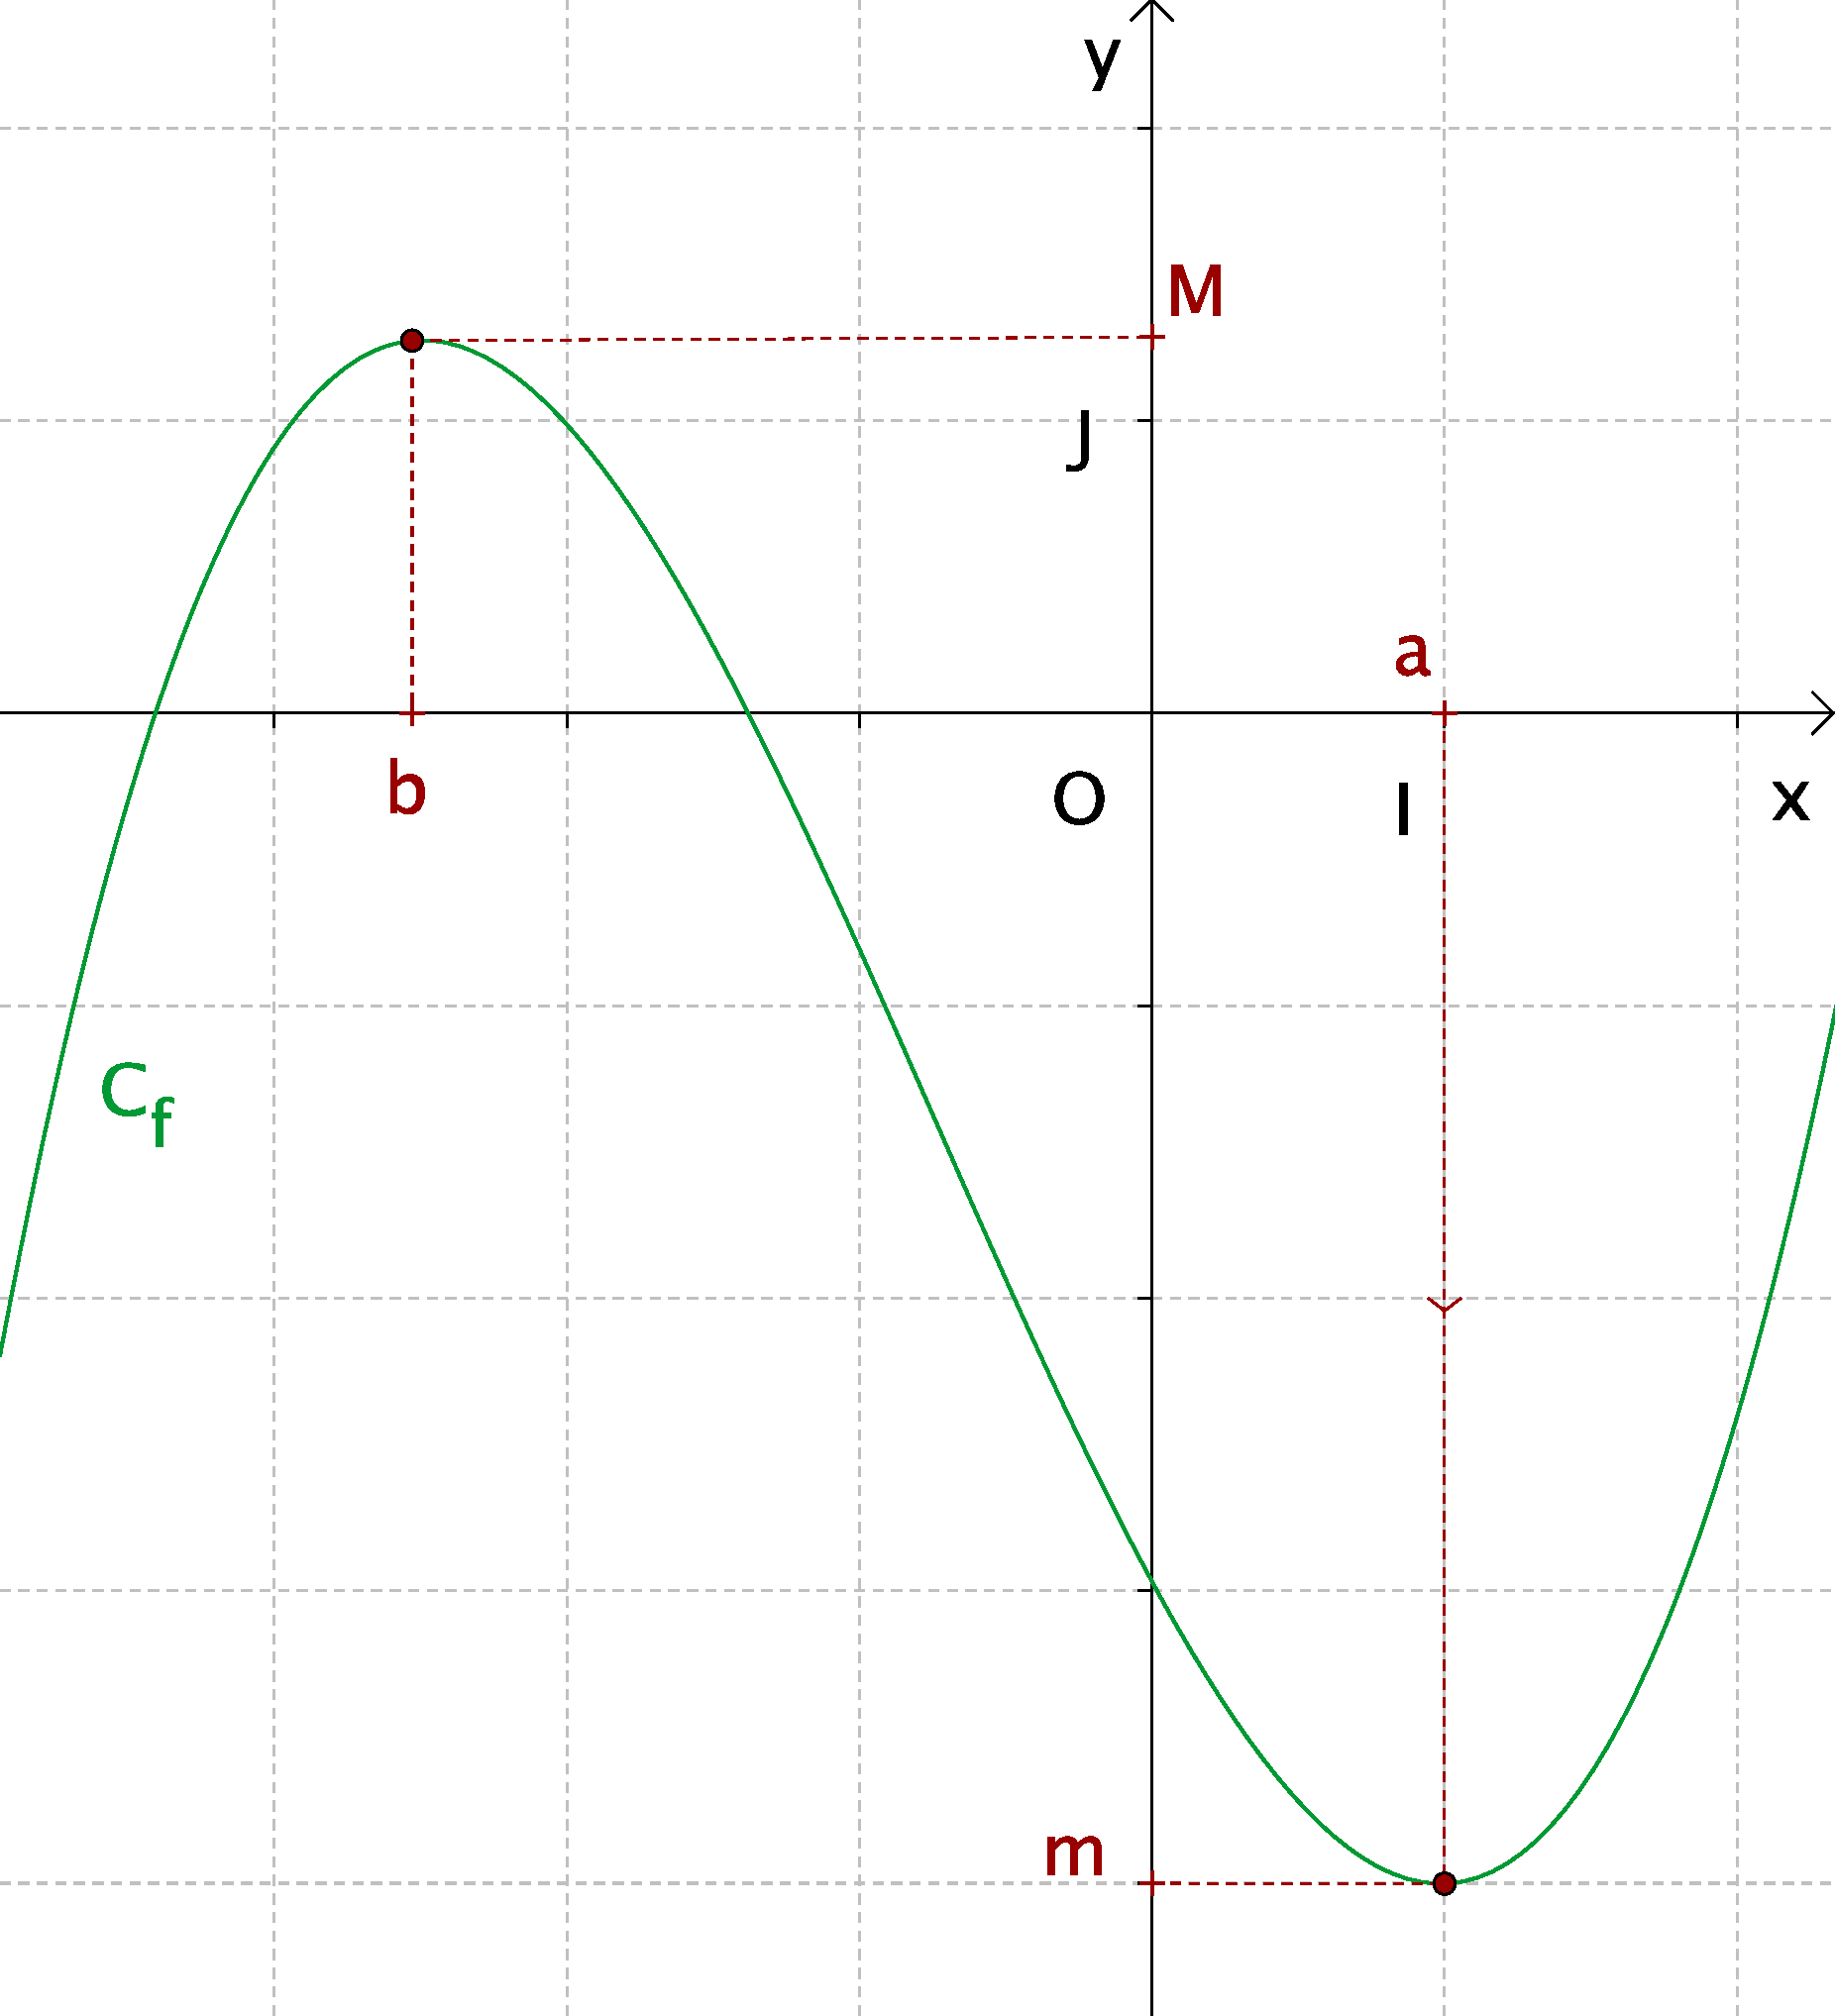
\includegraphics[width=6cm]{F_Extrema.pdf}
\end{minipage}
\quad
\begin{minipage}[c]{0.4\linewidth}
  \centering
  \ \\
  $f$ admet un \hspace{2cm} en $a$  \\[2ex]
  $\phantom{f(a)}a\approx$ \\[2ex]
  $\phantom{a}f(a)\approx $ \\[2em]
  
  \bigskip

  $f$ admet un \hspace{2cm} en $b$  \\[2ex]
  $\phantom{f(b)}b\approx$ \\[2ex]
  $\phantom{b}f(b)\approx $   
\end{minipage}



%+++++++++++++++++++++++++++++++++++++++++++++++++++++++++++++++++++++++++++++++++++++++++++++++++++++++++++++++++++++++++++
\section{Exercices à propos des fonctions}
%+++++++++++++++++++++++++++++++++++++++++++++++++++++++++++++++++++++++++++++++++++++++++++++++++++++++++++++++++++++++++++

\Exo{Seconde-0042}
\Exo{Seconde-0043}
\Exo{Seconde-0048}

\Exo{Seconde-0057}
\Exo{Seconde-0051}
\Exo{Seconde-0050}


\Exo{Seconde-0061}
\Exo{Seconde-0054}
\Exo{Premiere-0018}                                                                                                                                
\Exo{Seconde-0052}
\Exo{Seconde-0049}
\Exo{Seconde-0044}
\Exo{Seconde-0060}
\Exo{Seconde-0058}
\Exo{Seconde-0059}
\Exo{Seconde-0047}
\Exo{Seconde-0046}

